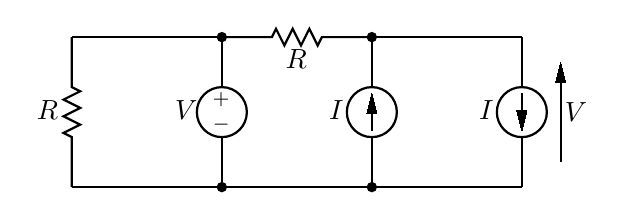
\begin{tikzpicture}[scale=2.54]
% dpic version 2020.06.01 option -g for TikZ and PGF 1.01
\ifx\dpiclw\undefined\newdimen\dpiclw\fi
\global\def\dpicdraw{\draw[line width=\dpiclw]}
\global\def\dpicstop{;}
\dpiclw=0.8bp
\dpiclw=0.8bp
\dpicdraw (0,0)
 --(-0,0.25)
 --(-0.041667,0.270833)
 --(0.041667,0.3125)
 --(-0.041667,0.354167)
 --(0.041667,0.395833)
 --(-0.041667,0.4375)
 --(0.041667,0.479167)
 --(0,0.5)
 --(0,0.75)\dpicstop
\draw (-0.041667,0.375) node[left=-2bp]{$ R_{\opx}$};
\dpicdraw (0,0.75)
 --(0.75,0.75)\dpicstop
\dpicdraw (0.75,0.75)
 --(1,0.75)
 --(1.020833,0.791667)
 --(1.0625,0.708333)
 --(1.104167,0.791667)
 --(1.145833,0.708333)
 --(1.1875,0.791667)
 --(1.229167,0.708333)
 --(1.25,0.75)
 --(1.5,0.75)\dpicstop
\draw (1.125,0.708333) node[below=-2bp]{$ R_{\opth}$};
\dpicdraw (1.5,0.75)
 --(2.25,0.75)\dpicstop
\dpicdraw (2.25,0.75)
 --(2.25,0.5)\dpicstop
\dpicdraw (2.25,0.375) circle (0.049213in)\dpicstop
\filldraw[line width=0bp](2.225,0.38125)
 --(2.25,0.28125)
 --(2.275,0.38125) --cycle\dpicstop
\dpicdraw (2.25,0.46875)
 --(2.25,0.304156)\dpicstop
\dpicdraw (2.25,0.25)
 --(2.25,0)\dpicstop
\draw (2.125,0.375) node[left=-2bp]{$ I_{\opout}$};
\filldraw[line width=0bp](2.469185,0.525)
 --(2.444185,0.625)
 --(2.419185,0.525) --cycle\dpicstop
\dpicdraw (2.444185,0.602094)
 --(2.444185,0.125)\dpicstop
\draw (2.444185,0.363547) node[right=-2bp]{$ V_{\opout}$};
\dpicdraw (2.25,0)
 --(1.5,0)\dpicstop
\dpicdraw[fill=black](1.5,0) circle (0.007874in)\dpicstop
\dpicdraw (1.5,0)
 --(1.5,0.25)\dpicstop
\dpicdraw (1.5,0.375) circle (0.049213in)\dpicstop
\filldraw[line width=0bp](1.525,0.36875)
 --(1.5,0.46875)
 --(1.475,0.36875) --cycle\dpicstop
\dpicdraw (1.5,0.28125)
 --(1.5,0.445844)\dpicstop
\dpicdraw (1.5,0.5)
 --(1.5,0.75)\dpicstop
\draw (1.375,0.375) node[left=-2bp]{$ I_{\opx}$};
\dpicdraw[fill=black](1.5,0.75) circle (0.007874in)\dpicstop
\dpicdraw (1.5,0)
 --(0.75,0)\dpicstop
\dpicdraw[fill=black](0.75,0) circle (0.007874in)\dpicstop
\dpicdraw (0.75,0)
 --(0.75,0.25)\dpicstop
\dpicdraw (0.75,0.375) circle (0.049213in)\dpicstop
\draw (0.75,0.3125) node{$_-$};
\draw (0.75,0.4375) node{$_+$};
\dpicdraw (0.75,0.5)
 --(0.75,0.75)\dpicstop
\draw (0.625,0.375) node[left=-2bp]{$ V_{\opx}$};
\dpicdraw[fill=black](0.75,0.75) circle (0.007874in)\dpicstop
\dpicdraw (0.75,0)
 --(0,0)\dpicstop
\end{tikzpicture}
